\section{Introdução}
\subsection{Teoria da Informação}
\begin{frame}%[allowframebreaks]
  \frametitle{Teoria da Informação e Codificação}

    \begin{itemize}[<+->]
    \item Surgiu em 1948 com a publicação do trabalho ``The Mathematical Theory of Communications'' \cite{shannon1948}.
    \item Teoria da Informação lida com as limitações teóricas e potencialidades de sistemas de comunicação.
    \item O que é informação? Como mensurar?
    \item Codificação. Como representar uma informação?
    \item Canal de Comunicação.
    \end{itemize}

\end{frame}
\note{
    \small
    \begin{itemize}
	\item A distinguibilidade entre as mensagens é fator importante para caracterizar informação.
        Pela definição de Shannon, ``Informação é a habilidade de distinguir de forma confiável
        dentre um rol de alternativas possíveis''.
	\item Shannon cunhou o termo `auto-informação' de um evento ou mensagem aleatória definindo-o como
	``menos o logaritmo da probabilidade do evento aleatório''. A `entropia' da fonte estocástica
	que gera os eventos é o valor esperado da auto-informação.
	\item Shannon mostrou que a entropia de uma fonte estocástica possui um significado físico:
	em média, é o menor número de bits necessários para representar ou comunicar de forma fidedigna 
	eventos gerados por uma fonte estocástica.
	\item O problema central em Teoria da Informação é a transmissão eficiente e confiável de dados, 
	do transmissor a um receptor, através de um canal de comunicação.
	\item Eficiência (usar o mínimo de recursos possível).
	\item Confiabilidade (evitar erros, ser capaz de detectá-los e corrigi-los).
    \end{itemize}
}
\note{
    \small
    \begin{itemize}    
	\item A informação é um conceito paradoxal. Por um lado necessita de uma representação física,
        por outro lado é abstrata. Uma mesma informação pode ser representada em papel,
        em um meio magnético ou ótico, pode ser representada por ondas mecânicas ou elétricas.
        \item Linguagem. Comunicação falada e escrita. Código faz associação entre símbolo e mensagem
	e é `arbitrário'.
    \end{itemize}
}
\note{
    \small
    A área da ciência criada por Shannon ampliou-se ao longo do tempo e influência diversas outras áreas.
    Por exemplo: teoria da comunicação, criptografia, ciência da computação, física (mecânica estatística),
    matemática (probabilidade e estatística), filosofia da ciência, linguística e processamento de linguagem natural,
    reconhecimento de fala, reconhecimento de padrões e aprendizado de máquina, compressão de dados, economia,
    biologia e genética, psicologia, etc.

    \vspace{3ex}
    Shannon entrou para o Bell Labs para trabalhar com sistemas de controle de disparo
    e criptografia durante a Segunda Guerra Mundial, sob um contrato com o Comitê Nacional de Pesquisa para Defesa
    Em 1945, Shannon elaborou um memorando sigiloso, que posteriormente foi publicado sob o título
    ``Communication Theory of Secrecy Systems''. Este incorporava muitos dos conceitos e formulações matemáticas
    do artigo mais consagrado ``A Mathematical Theory of Communication'' (1948).
}
\note{
    \small
    \begin{itemize}	
	\item Codificação - criar códigos com algoritmos práticos para codificação e decodificação para
	serem utilizados na comunicação no mundo real em canais ruidosos.
	\item Exemplos de codificações conhecidas para representar informação: código Morse, código ASCII, etc.
    \end{itemize}
}

\begin{frame}%[allowframebreaks]
  \frametitle{Código Morse}
  \hvFloat[floatPos=htb,capPos=right,capVPos=bottom,objectPos=c]{figure}{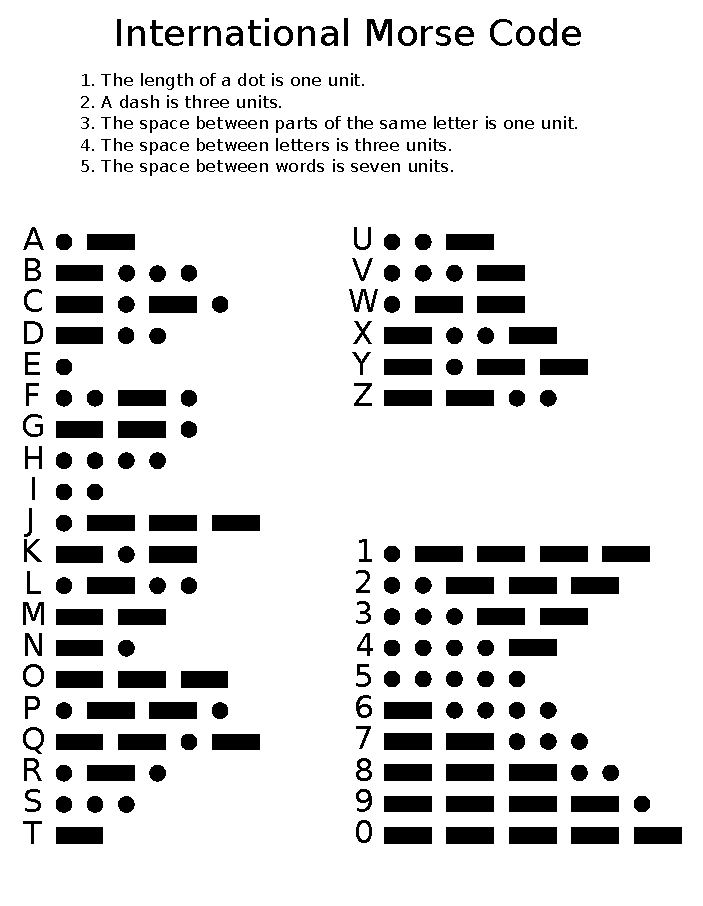
\includegraphics[trim=0cm 0cm 0cm 3.5cm,clip=true,width=0.45\textwidth]{images/International_Morse_Code.pdf}}
  {Código Morse internacional (\cite{wiki:morse}). Letras do alfabeto ordenadas por frequência de ocorrência no inglês: etaoin shrdlu cmfwyp vbgkjq xz (\cite{wiki:etaoin,wiki:letterfreq}).}{fig:morse}
\end{frame}

\begin{frame}%[allowframebreaks]
  \frametitle{Código Unário}
  Claude Mendibil utilizou o código unário (1, 01, 001, 0001, ...) 
  para representar as letras do alfabeto ESARINTULOMDPCFBVHGJQZYXKW.
  Utilizando este código, Jean-Dominique Bauby ditou o livro \textit{Le Scaphandre et le Papillon} (O Escafandro e a Borboleta).
  \hvFloat[floatPos=htb,capPos=right,capVPos=bottom,objectPos=c]{figure}{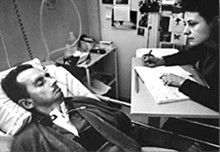
\includegraphics[width=0.45\textwidth]{images/bauby.jpg}}
  {Foto de Bauby em 1996 ditando suas memórias para Claude Mendibil (\cite{wiki:bauby}).}{fig:bauby}
\end{frame}

\begin{frame}%[allowframebreaks]
  \frametitle{Compressão}
  \begin{itemize}[<+->]
  \item Compressão é importante para utilizarmos melhor os recursos disponíveis.
  \item Shannon mostrou que o limite para a representação é a entropia.
  \end{itemize}
\end{frame}
\note{
  Compressão é importante para utilizarmos melhor os recursos disponíveis.
  \begin{enumerate}
  \item Armazenar mais dados em meio (disco rígido, memória, fita, etc).
  \item Transmitir mais informação através de um canal (essencialmente, armazenar e transmitir são o mesmo problema).
  \item Diminuir o desgaste do meio ao reduzir o número de vez que se faz leitura e escrita.
        Solid State Drives (SSDs) baseados em memórias flash NAND possuem um número finito de
        ciclos de programar/apagar. É importante reduzir a quantidade de bits que serão gravados para
        aumentar a vida útil dessas memórias/discos. (A compressão LZ4 vem sendo utilizada com esta finalidade, 
        e também para que o S.O. tenha um boot mais rápido)
  \end{enumerate}
}



\subsection{Modelo Geral de Comunicação}

\begin{frame}%[allowframebreaks]
  \frametitle{Modelo Geral de Comunicação}
  \begin{figure}[h!]
  \centering
  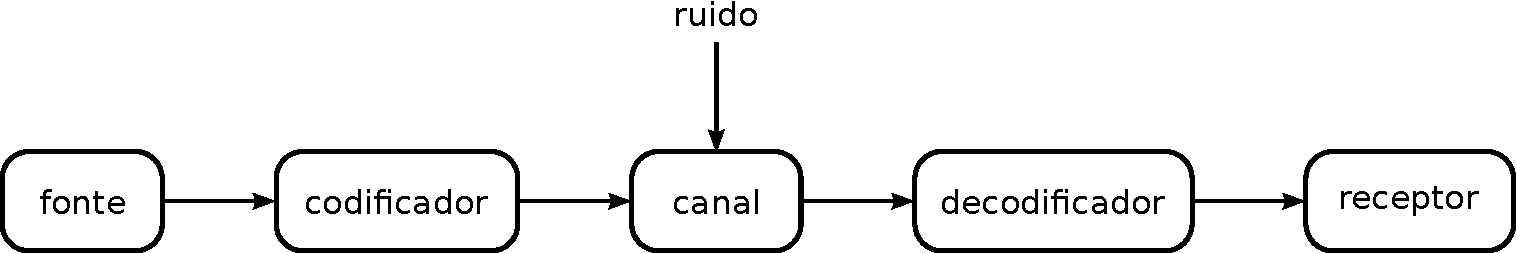
\includegraphics[width=\textwidth]{images/modelo-comunicacao.pdf}
  %\caption{.}
  \label{fig:modelo-comunicacao}
  \end{figure}
  \begin{description}
  \item[fonte] produz o sinal original que desejamos comunicar com um receptor;
  \item[codificador] modifica o sinal tornando-o mais apropriado para a comunicação;
  \item[canal] meio através do qual a mensagem será comunicada;
  \item[decodificador] faz o papel contrário do codificador, buscando recuperar a mensagem original;
  \item[receptor] receberá a mensagem enviada no processo de comunicação.
  \end{description}
\end{frame}
\note{
  \begin{itemize}
  \item Separação do codificador/decodificador em duas partes: codificador/decodificador de fonte e 
        codificador/decodificador de canal.
  \item Remover redundância do sinal produzido pela fonte e acrescentar redundância por causa 
        do ruído no canal de comunicação.
  \item Fontes e Canais de comunicação: discretos ou contínuos.
  \end{itemize}
}
\note{
  No contexto de Teoria da Informação, fonte é qualquer coisa que produza uma mensagem, um sinal que carregue informação.
  Podemos considerar uma fonte que produz mensagens como: voz, sons, palavras, imagens, 
  vídeo, sequência de bits de um programa de computador, etc.
}
\note{
  Canal é o meio através do qual o sinal produzido pela fonte será transmitido/propagado/armazenado.
  Por exemplo: espaço aberto (ar), linha telefônica, link de rádio, link em uma comunicação espacial,
  disco rígido, CD, DVD, fita magnética (armazenamento - transmissão no tempo ao invés de espaço pode 
  sofrer deterioração ao longo do tempo); DNA de seres vivos ao longo de gerações,
  envio de mensagens por estímulos elétricos ou químicos em um organismo biológico.
}
\note{
  Receptor é aquele a quem é destinada a mensagem transmitida. 
  Exemplos: computador ou equipamento, uma pessoa, rádio, tv, sistema de áudio, etc.
}
\note{
  Ruído é qualquer sinal que interfere com aquele que está sendo transmitido.
  Exemplos: ruído térmico, ruído impulsivo, cross-talk, outro sinal qualquer indesejado.
  Ruído representa a nossa compreensão imperfeita do universo. Desta forma,
  tratamos ruído como algo aleatório e que usualmente obedece certas regras, tais como
  uma determinada distribuição probabilística.
}
\note{
  O codificador processa o sinal antes de inseri-lo no canal de comunicação.
  \begin{itemize}
  \item Redução dos dados, removendo redundância do sinal.
  \item Inserção de redundâncias de acordo com as características do canal de comunicação, para 
  garantir integridade aos dados transmitidos.
  \item Codificação para representar as informações de um sinal sob a forma de outro sinal.
  \end{itemize}
}
\note{
  O decodificador faz o papel inverso do codificador.
  \begin{itemize}
  \item Remove os erros de transmissão.
  \item Recupera a informação original enviada pela fonte.
  \end{itemize}
}





\subsection{Notação}

\begin{frame}%[allowframebreaks]
  \frametitle{Notação}
   \begin{description}
   \item[$X$] é uma variável aleatória
   \item[$x$] é uma valor que a v.a. assume
   \item[$\mathcal{X}$] é o alfabeto de tamanho $\vert \mathcal{X} \vert = K$ dentro do qual a v.a. assume valores, $\mathcal{X} = \{a_1, \ldots, a_K\}$
   \item[$\mathcal{P}_X$] é o conjunto de probabilidades associadas aos valores, $\mathcal{P}_X = \{p_1, \ldots, p_K\}$, tais que $p_i \geq 0$ e $\sum_{i=1}^K p_i = 1$
   \item[$p_i$] é a probabilidade da v.a. assumir um determinado valor, $p_i = \Pr(X=a_i)$
   \item[$\mathcal{P}_X = p$] é a distribuição da v.a., $\sum_{x \in \mathcal{X}} \Pr(X=x) = 1$
   \item[$X \sim p$], a v.a. $X$ possui distribuição $p$
   \end{description} 
\end{frame} 
